\chapter{Implementazione}

\section{Protocolli di comunicazione}

REST+TCP+TLS

\section{Criticità}

Criticità nel normale esercizio del sistema, come la disconnessione di un Raspberry dalla rete, sovraccarico del server, led si fulmina (teoricamente è possibile accorgersene? Se no, lo togliamo).

\section{Implementazione della parte embedded}

\subsection{Configurazione dei Raspberry Pi}

Per quanto riguarda la scelta del sistema operativo da utilizzare, la scelta è ricaduta sulla distribuzione Linux Raspbian.
Questo perché è l'unica distribuzione ufficialmente supportata, ma anche perché, basandosi su Debian, offre un livelli di stabilità e sicurezza elevati.
Dato che i Raspberry dovranno essere dislocati sul territorio e collegati in rete, avere un adeguato livello di stabilità e sicurezza sono due tra le principali priorità.

Nonostante questa scelta il progetto è in grado di essere eseguito anche su una qualsiasi altra distribuzione Linux semplicemente installando tutte le dipendenze necessarie che verranno utilizzane in fase di implementazione del progetto.

I messaggi che i Raspberry Pi inviano quando comunicano con il server contengono al loro interno anche un timestamp per fini statistici.
Per evitare che con il tempo l'ora vada fuori sincrono si è impostato l'aggiornamento con \textit{ntp} giornalmente invece che, come di default, ad ogni avvio.
Questo perché i Raspberry Pi una volta dislocati sul territorio rimarranno sempre accesi senza effettuare mai riavvii a meno che non si presentino dei problemi.


\subsection{Linguaggio di programmazione, paradigma ad attori e organizzazione a task}

Per il programma in esecuzione sui Raspberry Pi si è scelto di utilizzare Python 3 che garantisce un elevato supporto per i sensori e attuatori attualmente disponibili.

Il paradigma ad attori è un modello matematico di computazione concorrente che tratta gli attori come primitive della computazione concorrente.
In risposta ad un messaggio ricevuto un attore può: effettuare una decisione locale, creare nuovi attori, inviare ulteriori messaggi, e determinare come rispondere al successivo messaggio che potrà ricevere. 

Dato che il software dei Raspberry è composto da diverse parti tra loro autonome e concorrenti, si è scelto di adottare il paradigma ad attori perché meglio rappresenta la struttura interna del progetto.
In questo modo ogni sottoparte è un attore e la comunicazione avviene solo tramite scambio di messaggi.
A tale scopo si è utilizzata la libreria \textit{pykka}.

Come visto in fase di progettazione, i Raspberry devono poter eseguire diverse operazioni concorrentemente, tra cui:

\begin{itemize}
	\item Rimanere in ascolto per eventuali richieste REST.
	\item Controllo presenza auto.
	\item Rilevamento intensità luminosa.
	\item Gestione illuminazione dei lampioni seguendo lo scheduling.
\end{itemize}

Per questo motivo è stata utilizzata la libreria \textit{threading} di Python che permette ad un singolo programma l'esecuzione di più thread.

\subsection{Controllo presenza auto \label{cpa}}

Per controllare la presenza di auto sulla carreggiata viene effettuato il calcolo della distanza utilizzando il sensore ad ultrasuoni HC-SR04. Per mitigare eventuali errori grossolani nella misurazione vengono effettuate sempre due misurazioni calcolando successivamente la media.

La misurazione avviene inviando un segnale ad ultrasuoni e calcolando il tempo che il segnale impiega per andare e tornare.
Per calcolare la distanza in centimetri si moltiplica il tempo per la velocità del suono nell'aria (34300 cm/s) e il tutto viene diviso per 2 perché il tempo era relativo all'andata e ritorno.

Per capire la direzione di marcia di un auto, nel caso di strade a doppio senso di marcia, è possibile adottare due strategie:
\begin{itemize}
	\item Posizionare nelle vicinanze del primo e dell'ultimo lampione, controllati da un determinato Raspberry, una coppia di sensori ad ultrasuoni a qualche centimetro di distanza tra essi.
	In questo modo controllando in che sequenza la coppia di sensori rileva la presenza di un auto è possibile intuirne la direzione di marcia.
	\item Posizionare in tutto due sensori ad ultrasuoni vicino ai lampioni controllati da un determinato Raspberry.
	Il primo andrà posizionato vicino al primo lampione sullo stesso lato della strada, e il secondo andrà vicino all'ultimo lampione sul lato opposto della strada.
	In questo modo impostando una soglia per il rilevamento delle auto pari al limite delle due carreggiate sarà possibile valutare il senso di marcia delle auto.
	Quindi per esempio, se il limite della carreggiata dista 2 metri dal bordo della strada, si imposterà il sensore in modo che se rilevi solo oggetti distanti meno di 2 metri, ed essi verranno considerate auto in transito sulla propria carreggiata.
\end{itemize}

Per l'implementazione di questo progetto si è optato per l'utilizzo della seconda strategia perché consente di ottenere lo stesso risultato utilizzando solo due sensori ad ultrasuoni invece che quattro.

L'utilizzo della prima strategia potrebbe tornare utile nel caso si voglia calcolare anche la velocità di crociera dei veicoli in transito.

In questo progetto essere in grado di capire il senso di marcia ci permette di accendere i lampioni in sequenza seguendo la direzione di percorrenza.

Il thread che si occupa del sensore di prossimità utilizza un secondo thread per inviare il segnale ad ultrasuoni.
Grazie a questa scelta si evita che il thread principale del sensore vada in busy waiting attendendo l'invio e il ritorno del segnale ad ultrasuoni.

Inoltre si è utilizzata la funzione \textit{wait\_for\_edge} che permette di fermare l'esecuzione del thread fino a quando non viene rilevata un'oscillazione, consumando una quantità irrisoria di CPU.

Di default il processo di misurazione considera la presenza di un veicolo sulla strada se la distanza rilevata è minore di 2 metri.
Tale valore può essere facilmente regolato in base alle caratteristiche della strada su cui si intende installare i sensori.

Il processo di controllo presenza auto è rappresentato da un attore il quale, dopo aver effettuato un controllo, notifica tutti i lampioni interessati.

\newpage
\lstinputlisting{code/ultrasonic.py}

\subsection{Rilevamento intensità luminosa}

Considerando che il Raspberry Pi non dispone di PIN analogici, per effettuare le letture di luminosità è possibile utilizzare le seguenti modalità:
\begin{itemize}
	\item Un sensore di luminosità digitale.
	\item Una fotoresistenza analogica collegandola ad un \textit{analog to digital converter (ADC)}
	\item Collegare un altro controllore che abbia pin analogici (e.g. arduino) e utilizzare una fotoresistenza analogica.
\end{itemize}

La terza modalità potrebbe essere presa in considerazione nel caso in cui si debba utilizzare diversi tipi di sensori analogici, tali da giustificare l'utilizzo di un controllore esterno.
Anche la seconda modalità può essere utile se si deve utilizzare più di un sensore analogico visto che un singolo ADC permette di utilizzare diversi pin analogici.

Nel nostro caso invece, dovendo collegare una singola fotoresistenza, si è optato per la prima modalità essendo la più semplice da attuare perché non richiede componenti aggiuntivi.
Per il progetto si è scelto di utilizzare il sensore digitale TSL2561.

In alternativa si potrebbe prevedere l'utilizzo di più sensori di luminosità in modo da essere in grado di effettuare una media delle letture, compensando eventuali letture errate dovute ad eventuali danneggiamenti o residui di sporco che potrebbero coprire il sensore.

Come per il controllo presenza auto della sezione \ref{cpa}, anche il processo di rilevamento è rappresentato da un attore.


\subsection{Scheduling illuminazione \label{si}}

Per quanto riguarda la programmazione dell'illuminazione il sistema offre la possibilità di impostare un'accensione, un inizio del periodo di risparmio energetico, uno spegnimento e una fine del periodo di risparmio energetico.
% in fase di progettazione è stato spiegato cos'è il periodo di risparmio energetico?
In tutte e quattro le impostazioni è previsto il campo relativo all'orario e alla soglia di intensità luminosa desiderata.

Si è deciso di dare la precedenza alla luminosità rilevata rispetto all'orario.
Questo comporta che nella pratica il funzionamento sarà il seguente:
\begin{itemize}
	\item Assumiamo di aver programmato l'accensione dei lampioni per le 19:00 con un livello di luminosità nell'ambiente pari a 50
	\item Se alle 19:00 l'intensità luminosa rilevata fosse minore di 50, i lampioni si accenderebbero.
	Invece nel caso in cui l'intensità luminosa fosse maggiore di 50 i lampioni rimarrebbero spenti nonostante siano le 19:00.
\end{itemize}

È stata effettuata questa scelta perché se la luminosità esterna fosse alta sarebbe poco utile accendere anche i lampioni, al contrario se la luminosità fosse bassa potrebbe anche essere dovuto a residui di sporco che con il tempo potrebbero depositarsi sul sensore.
Quindi anche se si rileva un livello di luminosità basso, si aspetta comunque l'orario impostato per accendere i lampioni.

La programmazione temporale viene espressa con precisione al minuto, visto che considerare anche i secondi sarebbe stata una precisione troppo elevata che sarebbe risultata non utile ai fini della programmazione.

La configurazione dei lampioni potrebbe essere salvata:
\begin{itemize}
	\item In locale su ogni dispositivo embedded o su un server centralizzato
	\item Utilizzando un database relazionale o un file di testo
\end{itemize}

Salvando le configurazioni su un server centrale si avrebbe il vantaggio di poter effettuare query consultando un singolo server.
Di contro però ogni dispositivo embedded dovrebbe sempre contattare il server per poter venire a conoscenza della propria programmazione e, nel caso in cui la connessione ad internet venisse a mancare, il dispositivo embedded smetterebbe di funzionare.

Salvando le configurazioni in locale su ogni dispositivo embedded si ha una maggiore resistenza ai guasti visto che, anche nel caso in cui la connessione internet venisse persa, il dispositivo embedded potrebbe continuare a funzionare essendo il proprio comportamento totalmente locale.

Un database relazionale offre prestazioni maggiori rispetto ad un file di testo, ma tale vantaggio sarebbe evidente solo nel caso in cui i dati da salvare siano in numero considerevole.
Un file di testo con una certa sintassi invece permette di controllare i valori salvati e di modificarli anche manualmente agendo direttamente sul file senza effettuare complicate query SQL.

Per questo si potrebbe preferire l'utilizzo di un database nel caso in cui si utilizzi un server centralizzato.
Se invece le configurazioni venissero salvate localmente sui singoli dispositivi embedded allora l'utilizzo di un RDBMS diventerebbe eccessivo e i pochi dati da salvare non ne giustificherebbero l'adozione.

Considerando i requisiti di progettazione come l'affidabilità del sistema e la facilità di gestione, si è scelto di salvare le configurazioni utilizzando un file di testo locale su ogni dispositivo embedded.
Inoltre il deploy dei dispositivi embedded potrebbe anche essere automatizzato ad esempio tramite l'utilizzo di un server ansible.

Grazie a questa scelta gli addetti ai lavori possono effettuare una programmazione agevole su ogni singolo lampione sia tramite interfaccia web che direttamente modificando i file di testo.

Per il formato con cui vengono salvate le configurazioni si è scelto di utilizzare il \textit{Configuration file parser} presente nelle librerie standard di Python perché permette la creazione di configurazioni con un linguaggio semplice, con una struttura simile ai file \textit{INI} di Microsoft Windows.
Questo garantisce una facile lettura e modifica anche manuale dei file.
I file così creati hanno una estensione \textit{cfg}.

I file hanno 4 sezioni principali con diversi campi ciascuna.
La prima sezione è \textit{GENERAL} e prevede tre campi:
\begin{itemize}
	\item \textit{lamp\_id}: Un identificativo intero progressivo del singolo lampione
	\item \textit{lamp\_pin}: Il numero del pin a cui il lampione è collegato sul dispositivo embedded
	\item \textit{lamp\_area}: L'zona di appartenenza del singolo lampione
\end{itemize}

La seconda sezione \textit{LampPolicyOn} e la terza \textit{LampPolicyOff} hanno gli stessi campi:
\begin{itemize}
	\item \textit{intensity}: L'intensità di luce del lampione espressa con un numero da 0 a 100. Impostando l'intensità a 0 equivale a spegnere il lampione.
	\item \textit{time\_h}: L'ora a cui questa impostazione dovrà iniziare
	\item \textit{time\_m}: Il minuto a cui questa impostazione dovrà iniziare
	\item \textit{photoresistor}: Il livello richiesto di luminosità ambientale
\end{itemize}

La quarta sezione è \textit{LampEnergySaving} e prevede cinque campi:
\begin{itemize}
	\item \textit{intensity}: L'intensità di luce del lampione espressa con un numero da 0 a 100.
	\item \textit{time\_h\_on} e \textit{time\_m\_on}: Rispettivamente l'ora e i minuti in cui inizia la modalità risparmio energetico.
	\item \textit{time\_h\_on} e \textit{time\_m\_on}:Rispettivamente l'ora e i minuti in cui finisce la modalità risparmio energetico.
\end{itemize}

Per una questione di coerenza l'inizio e la fine della modalità risparmio energetico deve essere obbligatoriamente compresa tra \textit{LampPolicyOn} e \textit{LampPolicyOff}.

In definitiva grazie a tale implementazione si è reso possibile sia la modifica dello scheduling di un singolo lampione con la comodità della interfaccia web, sia una modifica più avanzata collegandosi per esempio in SSH ad un Raspberry e cambiando i valori manualmente sui file di configurazione.

\lstinputlisting{code/light0.cfg}
\newpage

\subsection{Messaggi a fini statistici}

Quando i dispositivi embedded eseguono azioni rilevanti inviano ad un server centrale un messaggio \textit{json} per permettere agli addetti ai lavori di avere una panoramica generale sull'andamento dell'intero sistema.

I messaggi inviati contengono i seguenti campi \textit{json}:
\begin{itemize}
	\item "area": campo numerico che corrisponde alla zona di appartenenza del lampione. Serve a fini statistici per aggregare i dati.
	\item "action": è una stringa che può valere \textit{turn\_on}, \textit{turn\_off}, \textit{energy\_saving} o \textit{car\_detected}. Corrisponde al tipo di azione che è stata eseguita.
	\item "intensity": campo numerico relativo all'intensità di luce attuale del lampione
	\item "photoresistor": campo numerico relativo alla lettura della fotoresistenza.
	\item "timestamp": campo che contiene il timestamp in cui è avvenuta l'azione
\end{itemize}

\subsection{API REST}

Come scritto in fase di progettazione, i Raspberry Pi devono esporre un insieme di API di tipo REST per permettere di modificare le impostazioni relative alla programmazione dei lampioni.
Per tale scopo è stata utilizzata la libreria \textit{Flask}.

Quando un Raspberry riceve una richiesta tramite le API, per prima cosa vengono controllate le credenziali fornite perché è sempre richiesta una autenticazione tramite username e password per poter effettuare una qualsiasi GET o POST.

Se la richiesta ricevuta venisse valutata valida, verrà restituito un json, o con i dati richiesti o semplicemente con il codice 200, se la richiesta non prevedeva dati di ritorno.

%da rivedere e espandere

\subsection{Modalità Debug}

Per permettere agli addetti ai lavori di effettuare controlli sui lampioni, come per esempio verificare il loro corretto funzionamento, è stata prevista la possibilità di abilitare la modalità debug.

Entrando in modalità debug i lampioni si accenderanno e spegneranno in base ai comandi che verranno impartiti manualmente dagli addetti e ignoreranno le eventuali policy impostate in precedenza.

Per abilitarla è necessario inviare una richiesta POST di tipo REST all'indirizzo \textit{/debug/lamp/<int:lamp\_id>/on} oppure a \textit{/debug/lamp/<int:lamp\_id>/off}.
Rispettivamente il primo serve per accendere il lampione e il secondo per spegnerlo.
Le richieste POST dovranno contenere un campo \textit{intensity} che corrisponde all'intensità desiderata a cui si intende impostare il lampione.

Quando si vuole concludere la fase di debug bisogna inviare una POST all'indirizzo \textit{/debug/lamp/<int:lamp\_id>/stop}.
Una volta conclusa la fase di debug i lampioni torneranno a funzionare seguendo il proprio scheduling.

\section{Implementazione del Web Server REST}

Come scritto nella sezione \ref{si} per permettere agli addetti ai lavori di controllare e modificare la programmazione dei singoli lampioni è stata implementata una interfaccia Web tramite un server REST.

Come misura di sicurezza, tutte le richieste GET e POST ai Raspberry dovranno essere corredate da nome utente e password relativi al singolo dispositivo embedded che si intende contattare.
%(mmm, la storia del "dare ad un addetto solo le credenziali dei rpi della sua zona dove lo mettiamo?)

Il sito Web è stato realizzato seguendo uno stile minimale, moderno e il quanto più intuitivo per l'utente.
L'interfaccia è ottimizzata sia per un uso desktop che mobile.

\begin{figure}[tbp]
	\centering
	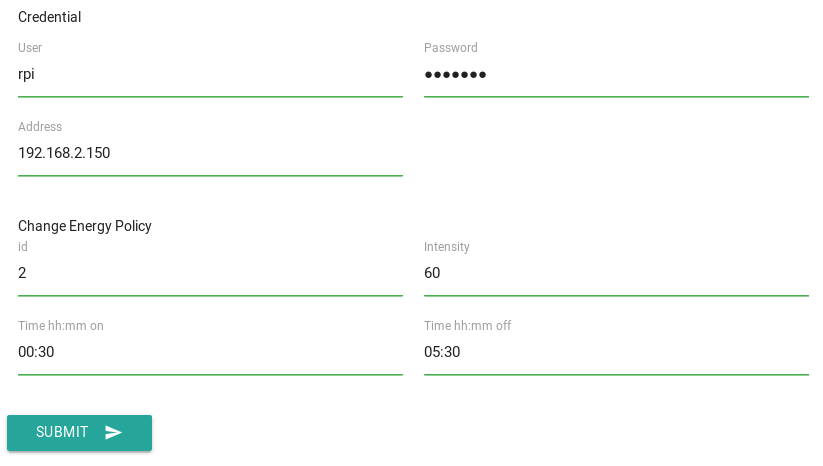
\includegraphics[scale=.62]{figure/web_desktop.png}
	\caption{Interfaccia web Desktop \label{FSM POLICY}}
	\subfloat[(Mobile) Campi corretti]{{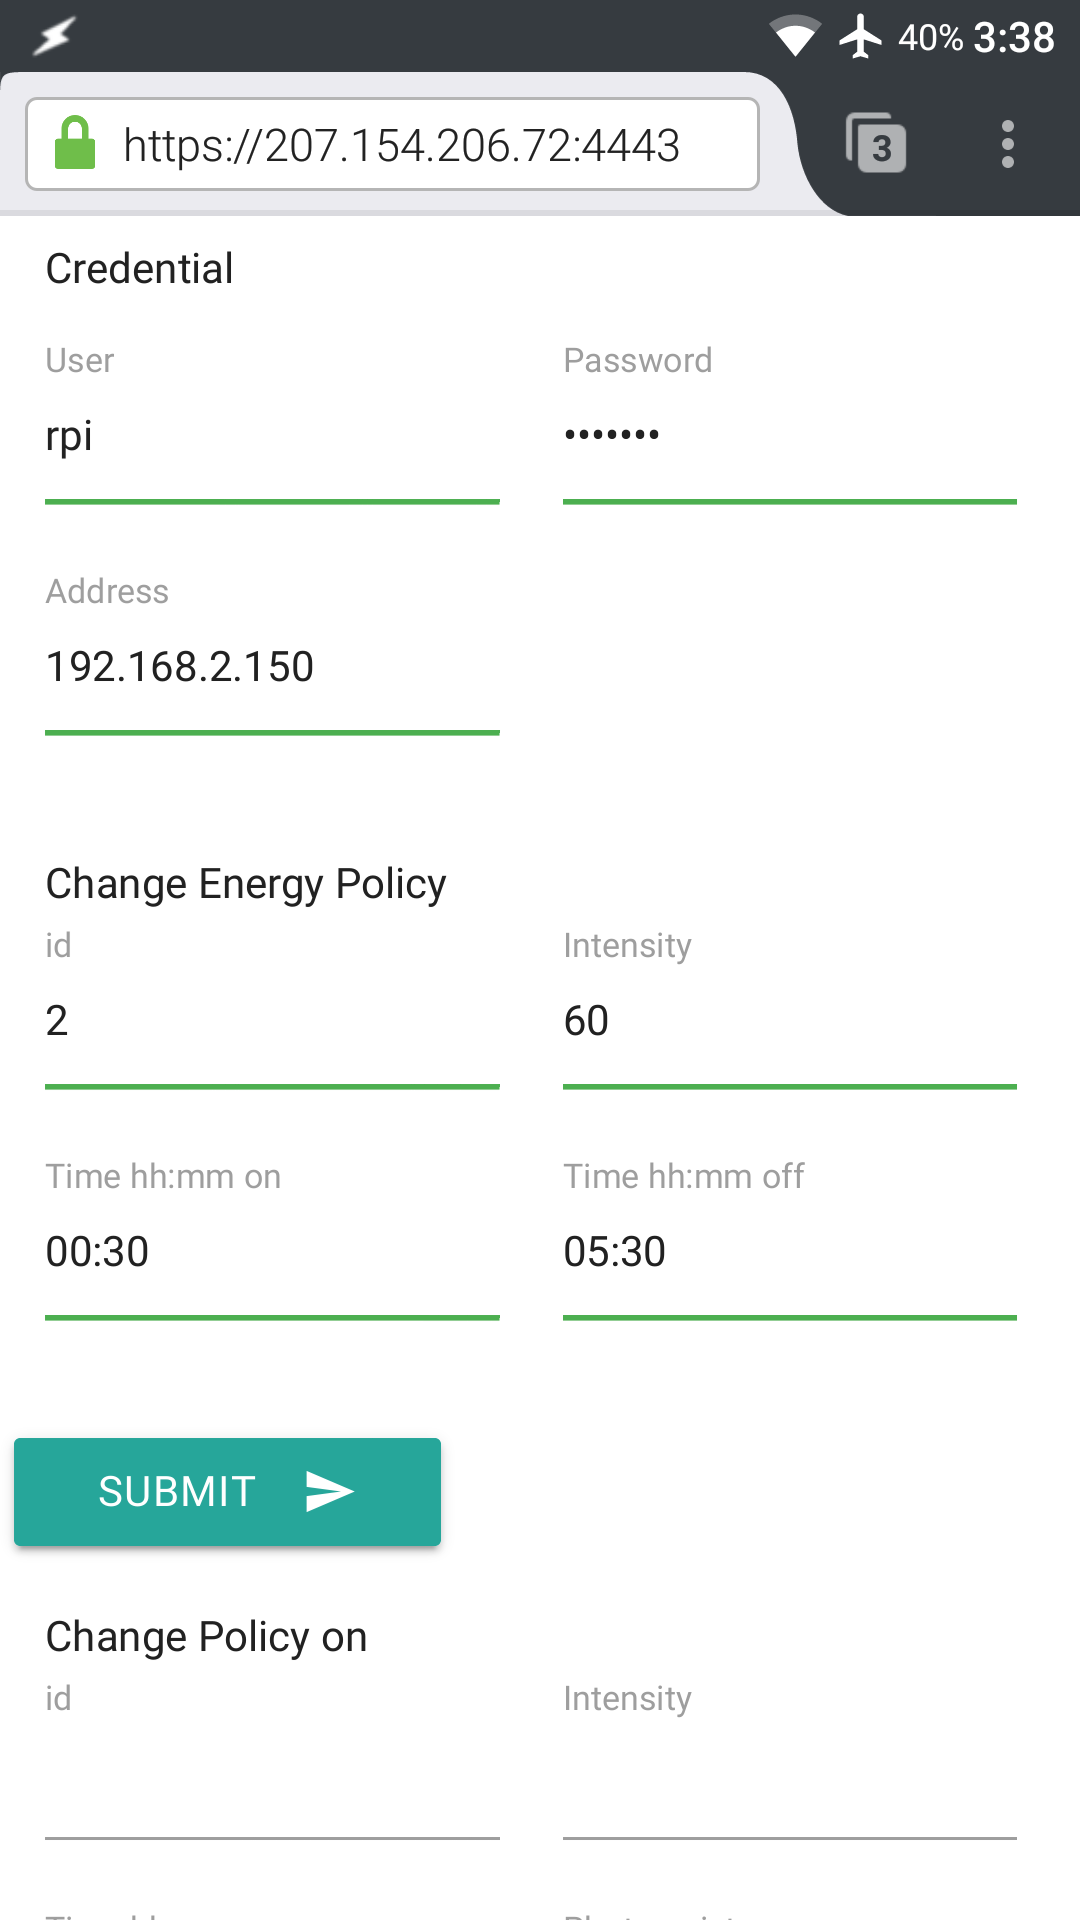
\includegraphics[width=6cm]{figure/web_mobile.png} }}%
	\qquad
	\subfloat[(Mobile) Campi mancanti o errati]{{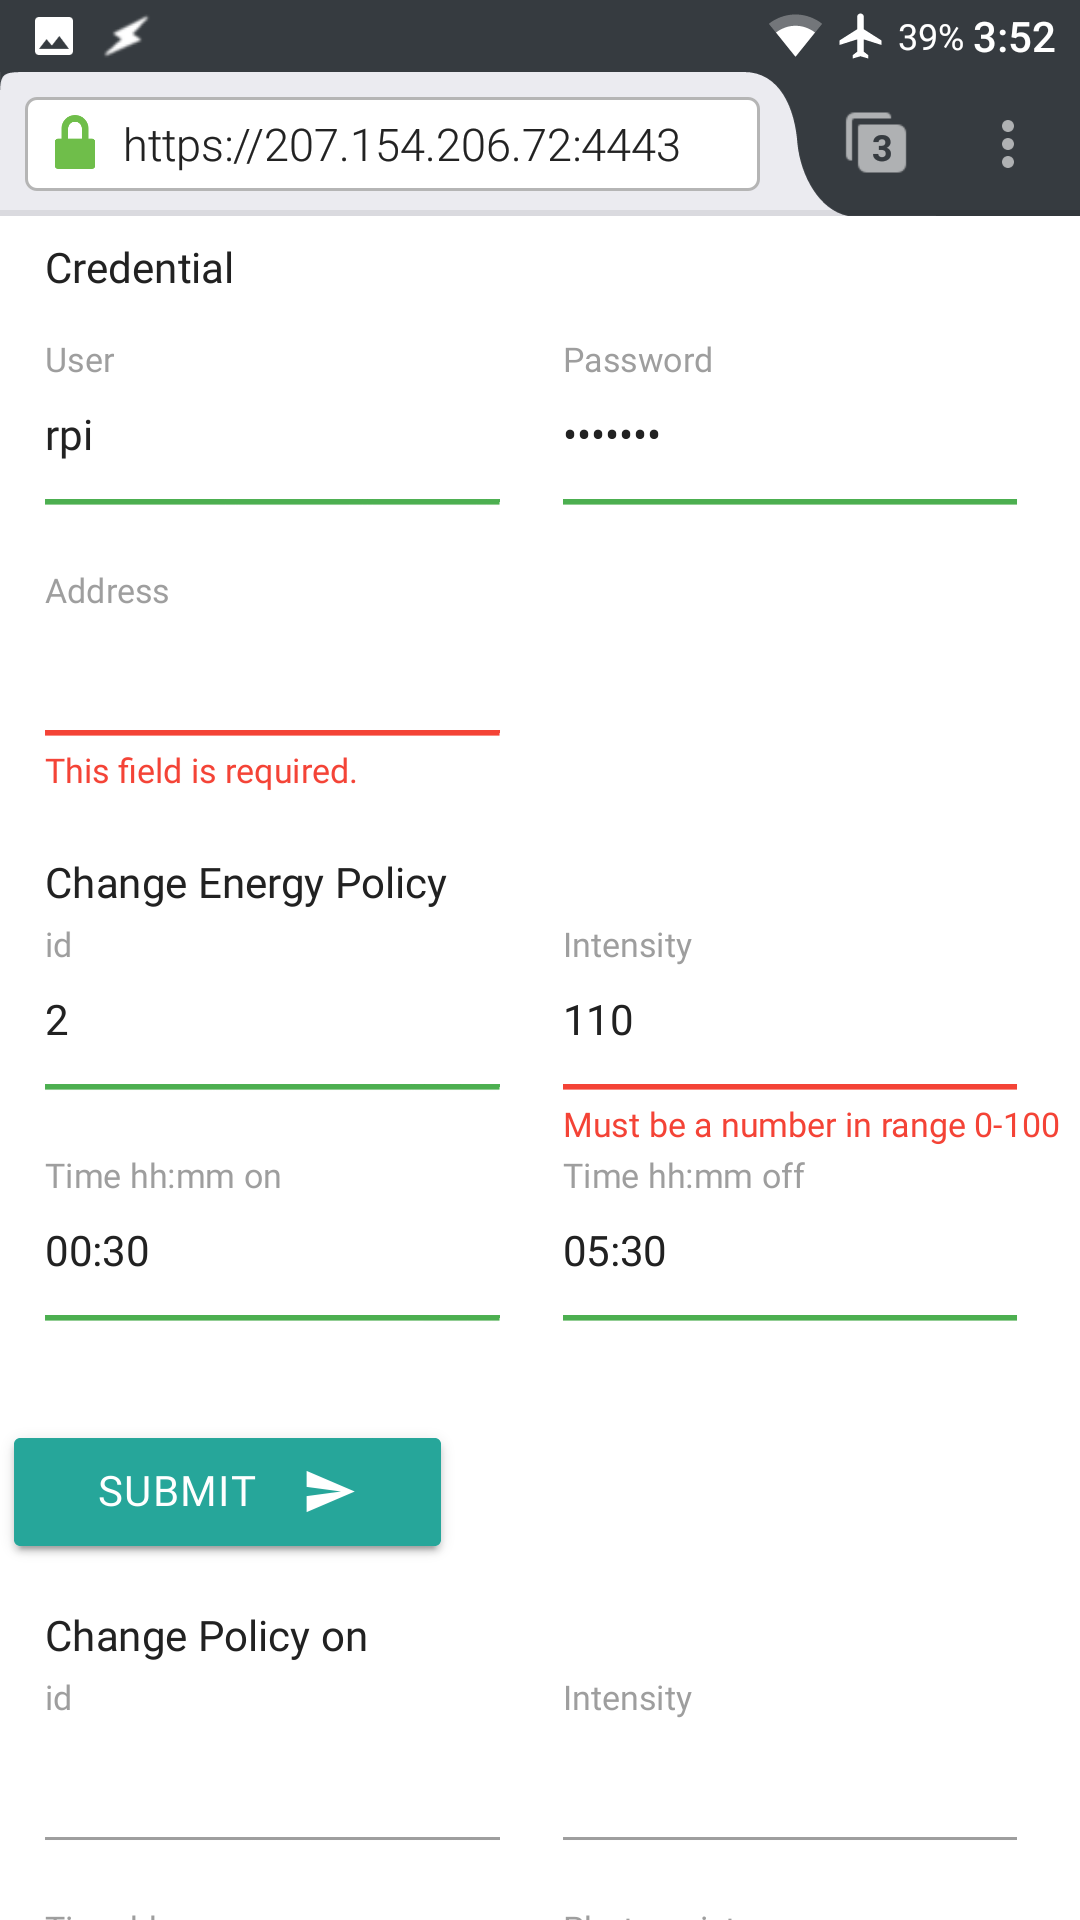
\includegraphics[width=6cm]{figure/web_mobile_errors.png} }}%
	%\caption{Esempi della interfaccia mobile}%
	\label{fig:example}%
\end{figure}

\newpage

\subsection{Linguaggi e librerie}

Il Web Server può essere realizzato dinamicamente, ad esempio tramite l'utilizzo di php, o staticamente.

Durante l'implementazione si è scelto di realizzarlo staticamente perché:
\begin{itemize}
	\item Il sito consiste in una singola pagina web che contiene sempre le stesse informazioni.
	\item Essendo le comunicazioni basate su REST, è il client a contattare direttamente il destinatario, mentre se il sito fosse dinamico, il server farebbe da intermediario.
	\item Evitando di utilizzare php si riduce anche il numero di possibili attacchi che il server potrebbe subire
	\item Visto che il sito è semplice, realizzandolo staticamente è più facile ottenere un design più pulito.
\end{itemize}

Per quanto riguarda lo \textit{style sheet language} due delle più comuni implementazioni sono l'utilizzo diretto di CSS o di uno strumento di automatizzazione come SASS.
Essendo il Web Server composto da un'unica pagina Web con un'interfaccia piuttosto semplice si è optato per l'utilizzo di CSS, perché SASS non sarebbe stato di particolare aiuto.

Per le motivazioni sopra elencate il Web Server è stato realizzato utilizzando i linguaggi HTML, CSS e JavaScript.
Per il CSS si è utilizzata la libreria \textit{materialize}, mentre per quanto riguarda JavaScript si è utilizzato \textit{JQuery} e \textit{JQuery validate} per effettuare controlli client side sui form compilati dagli utenti.


